% Research Paper for MICS 2014
% by David Donatucci, Kirbie Dramdahl, and Nic McPhee

\documentclass[12pt]{article}

\setlength{\oddsidemargin}{0in}
\setlength{\evensidemargin}{0in}
\setlength{\topmargin}{0in}
\setlength{\headheight}{0in}
\setlength{\headsep}{0in}
\setlength{\textwidth}{6in}
\setlength{\textheight}{9in}
\setlength{\parindent}{0in} 

\usepackage{parskip}
\usepackage{times} %For typeface
\usepackage{graphicx}
\usepackage{algorithm}
\usepackage{algorithm,algorithmic}
\usepackage[justification=centering]{caption}[2007/12/23]
\usepackage{url}
\sloppy

\usepackage{float}
\newfloat{Query}{tbp}{lop}

\newcommand{\inset}[1]{$\in \{ {#1} \}$}

\newcommand{\citep}[1]{\cite{#1}}
\newcommand{\PPLR}[1]{$\eta_M$}
\newcommand{\LLR}[1]{$\eta_L$}

\DeclareGraphicsRule{.tif}{png}{.png}{`convert #1 `dirname #1`/`basename #1 .tif`.png}

\title{Analysis of Genetic Programming Ancestry Using a Graph Database}

\author{
 		David Donatucci, M. Kirbie Dramdahl, and Nicholas Freitag McPhee\\
        Division of Science and Mathematics\\
        University of Minnesota, Morris\\
        Morris, MN 56267\\
        donat056@morris.umn.edu\\
        dramd002@morris.umn.edu\\
        mcphee@morris.umn.edu\\
}
\date{} 

\begin{document}
\pagestyle{plain}

\maketitle

\begin{abstract}

Genetic programming is an artificial intelligence technique that uses concepts from biological evolution such as fitness, mutation, and crossover to manipulate a population of functions, typically represented as trees. Analyzing the complex dynamics of such a system can be challenging. Researchers rarely save or analyze most of the intermediate data from a run, and instead focus on statistical summaries of generations. However, information is lost in this process, precluding potentially important analysis of key events during the run.

Our objective here is to use graph databases to store and analyze the ancestry of individuals. Graph databases are relatively new, and provide features such as queries to obtain data that would be difficult with relational databases. In relational databases, as data sets increase in size, recursive queries become extremely inefficient. By comparison, with a graph database such as Neo4j, the execution time for recursive queries remains relatively constant as the size of data sets grows. Since genetic programming involves a significant number of trees and a multitude of generations, graph databases allow for efficient querying of ancestry that would not be possible with more traditional database systems such as SQL.

Our hope is that by recording and analyzing tree ancestry, we will be able to obtain valuable insight into the evolutionary process of genetic programming. Perhaps most significantly, we hope to discover where trees show significant improvement in fitness and how those improvements are obtained. This will allow for a better understanding of how genetic programming works and provide details for future improvements in the evolutionary computation field.

\end{abstract}

\section{Introduction} \label{sec:intro}

Genetic programming (GP) is an artificial intelligence technique that uses concepts from biological evolution such as fitness, mutation, and crossover to discover solutions to user defined problems. Genetic programming manipulates populations of individuals which are evaluated based upon their fitness. Individuals providing the best solution to the target problem will have stronger fitnesses, and will typically produce more offspring than those with weaker fitnesses. Over many generations, descendants generally have stronger fitnesses than their ancestors from previous generations.

Genetic programming systems are great tools for discovering solutions to complex problems, especially those involving many variables that would be difficult to solve by other means. Genetic programming has applications in chemistry, electronic circuit design, economics, and many other areas. 

While evolutionary algorithms have clearly been successful in a variety of settings, it is often challenging to determine why this is true. In order to reach a greater understanding of the processes involved in genetic programming, it is necessary to examine the internal interactions of individuals within a run, rather than simply reporting statistical summaries of the final results. Even simple GP runs can generate very large data sets, however, especially if one records all the individuals and relationships from every generation.

Databases are a natural tool for handling such large data sets, but answering important questions and queries for GP work can be onerous when using relational databases. A natural question when analyzing an GP run, for example, would be to find all the ancestors of the ``winning'' individual. If we used a relational database, we might store the IDs of the parents along with each individual. A single query would then return the parents of an individual, but then additional queries (one per parent) would be needed to get the set of grandparents, and additional queries (one per grandparent) would be needed to get the set of great grandparents, etc. Assuming two parents per individual, the number of queries will then grow as $O(2^n)$ where $n$ is the number of generations we wish to examine, making this approach totally unfeasible for a host of interesting and important questions.

New graph database technologies, however, have the potential to allow us to easily perform these sorts of queries and analyze important dynamic properties of GP runs. In graph databases one stores nodes and relationships, such as individuals and their relationships to their parents, and the query language makes it easy to search for paths through the graph having specified properties. This makes it fairly trivial to ask important ancestry questions about a run; the query \texttt{MATCH (a)-[:PARENTOF*]->(d)}, for example, will find all the ancestors $a$ of some individual $d$. (The details of graph databases and the Cypher query language will be described in more detail in Section~\ref{sec:Graph Databases}.)

This paper demonstrates the usefulness of graph databases in recording and analyzing data produced by GP systems. A description of genetic programming is provided in Section~\ref{Genetic Programming}, and Section~\ref{sec:Graph Databases} discusses graph databases. Section~\ref{sec:experiments} provides details on how we set up our experimental runs. The results of our work are presented in Section~\ref{sec:results}, and ideas for future implementation and applications of this work are presented in Section~\ref{sec:conclusion}.

\section{Genetic Programming} \label{Genetic Programming}

Genetic programming~\cite{poli08:fieldguide} is based around the interactions of individuals. Individuals are similar to organisms in biological evolution. As in biological evolution, a group of individuals makes up a population. In the process of biological evolution and natural selection, organisms within a population compete in order to survive and reproduce. Those individuals best adapted to their environment have the best chance of fulfilling these objectives.  In genetic programming, individuals also compete, but here those individuals that provide better solutions to the user-defined target problem have the best odds. The goal of genetic programming is to produce individuals that provide quality solutions.

GP is commonly applied to symbolic regression problems, where the goal is to evolve a function that passes through a collection of test points, either coming from empirical data or a synthetic test problem. The fitness is then the difference between the target function and the function encoded by the individual. The lower the fitness, the better the solution fits the target problem, and an individual with a solution that perfectly fits the problem would have a fitness of zero. Therefore, at the conclusion of a genetic programming run, it is desirable to have one or more individuals with fitness at or near zero.

At the start of a run, the population is filled with randomly generated individuals. The individuals within this population then compete in order to pass their code on to the next generation, similar to biological evolution. In this work we used tournament selection, where a specified number of individuals are randomly chosen from the population, and those with the best fitness are selected to produce the next generation. These selected individuals can propagate their genetic material to the next generation by one of three transformation methods. The first and most common method is crossover, comparable to sexual reproduction, where two individuals are selected from the current generation, and elements from each selected individual are combined to form a new individual in the next generation. The second method is mutation, in which an individual is selected and randomly altered, much like biological mutation. The third and final method is reproduction, where an individual is copied to the next generation, akin to asexual reproduction. There is also an alternative form of reproduction known as elitism, where the best few individuals are copied to the next generation by merit of their fitness alone. Crossover, mutation, and reproduction are utilized many times, across multiple generations, until an ideal or approximate solution is found or until some sort of resource limit is reached.

\section{Graph Databases}
\label{sec:Graph Databases}

Graph databases~\cite{GraphDatabases:2013} are a relatively new approach, where data is stored as a collection of nodes and relationships in a graph, with a specialized query language that makes it easy to ask questions about complex relationships. We used the Neo4j graph database system to collect data generated by GP runs. This section further describes Neo4j, its query language Cypher, and the various advantages they hold over relational databases in recording and accessing information that relies heavily on recursion.

Neo4j is a form of data management system based upon a graph. Information is stored by means of vertices and edges, commonly referred to as nodes and relationships, respectively~\cite{GraphDatabases:2013}. In our work, nodes represent individuals, and relationships represent the transformations between individuals. As our GP system generates individuals, new nodes and relationships are added to the database for later analysis.

Cypher~\cite{GraphDatabases:2013} allows this data to be readily extracted from the Neo4j database. There are three fundamental elements to queries in Cypher. The \texttt{START} clause specifies a starting location in the database, indicating the node or nodes where the query will begin. The \texttt{RETURN} clause specifies which nodes, relationships, or properties should be returned to the user. The \texttt{MATCH} clause is the main section of a query, specifying what patterns in the graph the query will discover. To write the \texttt{MATCH} clause, nodes and relationships are drawn with ASCII characters. A node is indicated by parenthesis \texttt{( )}, directed relationships are indicated with \texttt{-->} or \texttt{<--} depending on the direction of the relationship, and undirected relationships are indicated with \texttt{--}. Brackets \texttt{[ ]} between the dashes can be used to specify relationship names prefixed by a colon. In the example query below, the \texttt{START} clause indicates that the query should start with node 43, called \texttt{parent}, the \texttt{MATCH} clause finds all nodes that are children of the starting node, and the \texttt{RETURN} clause yields the starting node and all nodes that are children of that node.

\begin{verbatim}
    START parent=node(43)
    MATCH (parent)-[:PARENTOF]->(child)
    RETURN parent, child;
\end{verbatim}

This query produces the results in Figure \ref{fig:exampleQuery}.
\begin{figure}[tb]
 \centering
 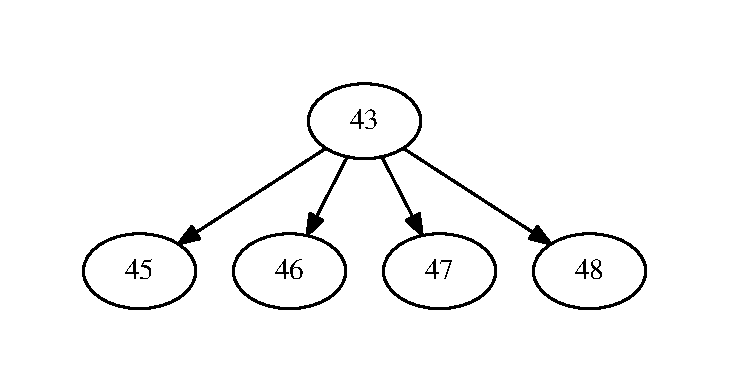
\includegraphics[height=0.30 \textwidth]{parents}
 \caption{Results of Example Query}
 \label{fig:exampleQuery}
\end{figure}

Performance is the key advantage in our research of graph databases over relational databases. As the data set grows, recursive queries such as those needed to explore graph relationships become highly inefficient when using relational databases, as numerous joins are needed. In graph databases, however, the portion of the data set that must be searched is limited because the query will only search along an available path connected by relationships, allowing queries to remain efficient~\cite{GraphDatabases:2013}.

\section{Experimental Setup} 
\label{sec:experiments}

This section explains the details of the configurations used for this research. Subsection~\ref{sec:GPSetup} covers setup of the genetic programming algorithm, and Subsection~\ref{sec:Neo4jSetup} discusses setup of the graph database Neo4j.

\subsection{Genetic Programming Setup}
\label{sec:GPSetup}

In our system, individuals contain two items: a function called the tree, and the tree's fitness. Trees are represented in prefix notation by arrays containing variables, constants, and operators. Prefix notation places the operator before its arguments. For example, the function $x + (x * 4)$ would be represented by the following array: $[+, x, *, x, 4]$. The tree's fitness is the sum over all the test cases of the absolute error between the target function $t$ and the function $f$ represented by the tree:
\[
	\textrm{fitness} = \sum_i |f(x_i)- t(x_i)|
\]

After the tree's fitness is computed, we add 1\% of the length of the array to the fitness as a means of penalizing particularly large trees. This combats the tendency for trees to become excessively large, and is commonly referred to in genetic programming as bloat control. This implementation of bloat control is relatively weak in the beginning of a run where trees usually have larger fitnesses (therefore not penalizing them unreasonably), but has a significant impact later in the run, where trees should have smaller fitnesses.

In all of the runs, the configurations remained consistent, with the exception of population size, which was either 1,000, or 10,000. The target function was $\sin(x)$,
where the value of the variable $x$ ranged from 0 to 6.2, increasing by steps of 0.1. The constants allowed were doubles that ranged between -5 and 5, and $x$ was the sole variable. The function set consisted of the binary operations: addition, subtraction, multiplication, and protected division. In our implementation of protected division, if the denominator equals zero, then regardless of the numerator, the output will be one. The reason we chose the output one for protected division is so there would not be a discontinuity in the function $x/x$ when $x = 0$, thus allowing individuals to use the expression $x/x$ to obtain the value one.

To create the initial population, we used the PTC2 algorithm~\cite{Luke2013Metaheuristics}. This creates trees by randomly adding operators to an array (leaving blank slots where appropriate for arguments) until a specified length is reached. The blank slots are then filled by leaves (variables and constants). In our system, leaves consist of 63\% variables and 37\% constants, following the proportions used in TinyGP~\citep{poli08:fieldguide}.

We used tournament selection to select those individuals which will produce the next generation. In our tournament, two individuals are chosen randomly from the entire generation. The individual with the best fitness of the two is then selected to propagate its code in some capacity to the next generation.

In our system, the top 1\% of the current generation is directly copied to the next generation via elitism. The remaining 99\% are created via three different means: crossover, mutation, and reproduction. Crossover makes up 90\% of all transformations, mutation 1\%, and reproduction accounts for the remaining 9\%. Reproduction is relatively straightforward, where the individual which wins the tournament is simply copied to the next generation. Mutation and crossover are more complex processes, and will be covered in the following paragraphs.

Mutation begins in a similar manner to reproduction. Two individuals are chosen from the population to enter the tournament, and the winner is selected for mutation. However, rather than simply copying this individual to the next generation, a random position in the tree is selected. The subtree rooted at that position is then removed and replaced by a new subtree generated by PTC2 that is at most half the size of the original tree. This limitation has been put in place to help control bloat.

Crossover differs from the previous transformations in that it makes two calls to tournament selection in order to select two parent individuals to produce a single child individual in the next generation. Within this parent, similar to mutation, a random position is chosen. The subtree rooted at that position is removed and replaced by a subtree randomly selected from the individual that won the second tournament. The first parent, which contributes the root node to the child, is called the \emph{root parent}; the second parent which contributes the subtree is called the \emph{non-root parent}.

\subsection{Neo4j Setup}
\label{sec:Neo4jSetup}

In Neo4j, we set nodes to be individuals and defined their ancestry as relationships. Inside each node, we inserted several attributes belonging to an individual. In addition to the tree and fitness, all nodes also include the penalized fitness, the generation number, the transformation type that generated this individual, the run id (used to differentiate between different runs), and a unique id (used for identifying the specific node). For individuals produced by either crossover or mutation, the ``cut point'' (the position at which the root parent was altered by a transformation) is also included as an attribute.

Each individual has a relation to its parent (or parents in the case of crossover). To distinguish between each type of transformation, different types of relationships are used. These relationships are demonstrated in Table~\ref{tab:relationshipTypes}.
\begin{table}[tb]
\begin{center}
\begin{tabular}{|l|l|}
    \hline
    \multicolumn{2}{|c|}{\textbf{Relationship Types}} \\
    \hline
    Reproduction & PARENTOF \\
    Elitism & ELITISM \\
    Mutation & MUTANTOF \\
    Crossover Root & ROOT\textunderscore XOOF \\
    Crossover Non-Root & NONROOT\textunderscore XOOF \\
    \hline
\end{tabular}
\caption{On the left are the various transformation types and on the right are the relationship types assigned to each in the Neo4j database. Notice that crossovers have two types of relationships to distinguish between the root parent and the non-root parent.}
\label{tab:relationshipTypes}
\end{center}
\end{table}

\section{Results} \label{sec:results}

To obtain the results presented here, we completed three runs using population size 1,000, and one using population size 10,000. The average size of the database for the 1,000 individual runs was 380Mb, and the size of the database for the 10,000 individual run was 3.7Gb.

From these runs, we were able to perform a variety of interesting queries. Most queries completed in a manner of seconds; some of the more complex queries took up to 15 minutes. Computing, for example, the root ancestry path (explained below; see Figure~\ref{fig:XO_path_example}) for an individual in the final generation took roughly 1 second for both the 1,000 individual results and the 10,000 results, whereas that sort of recursive query would almost certainly be much slower on the larger database using a relational system such as SQL.

\begin{figure}[tb]
 \centering
 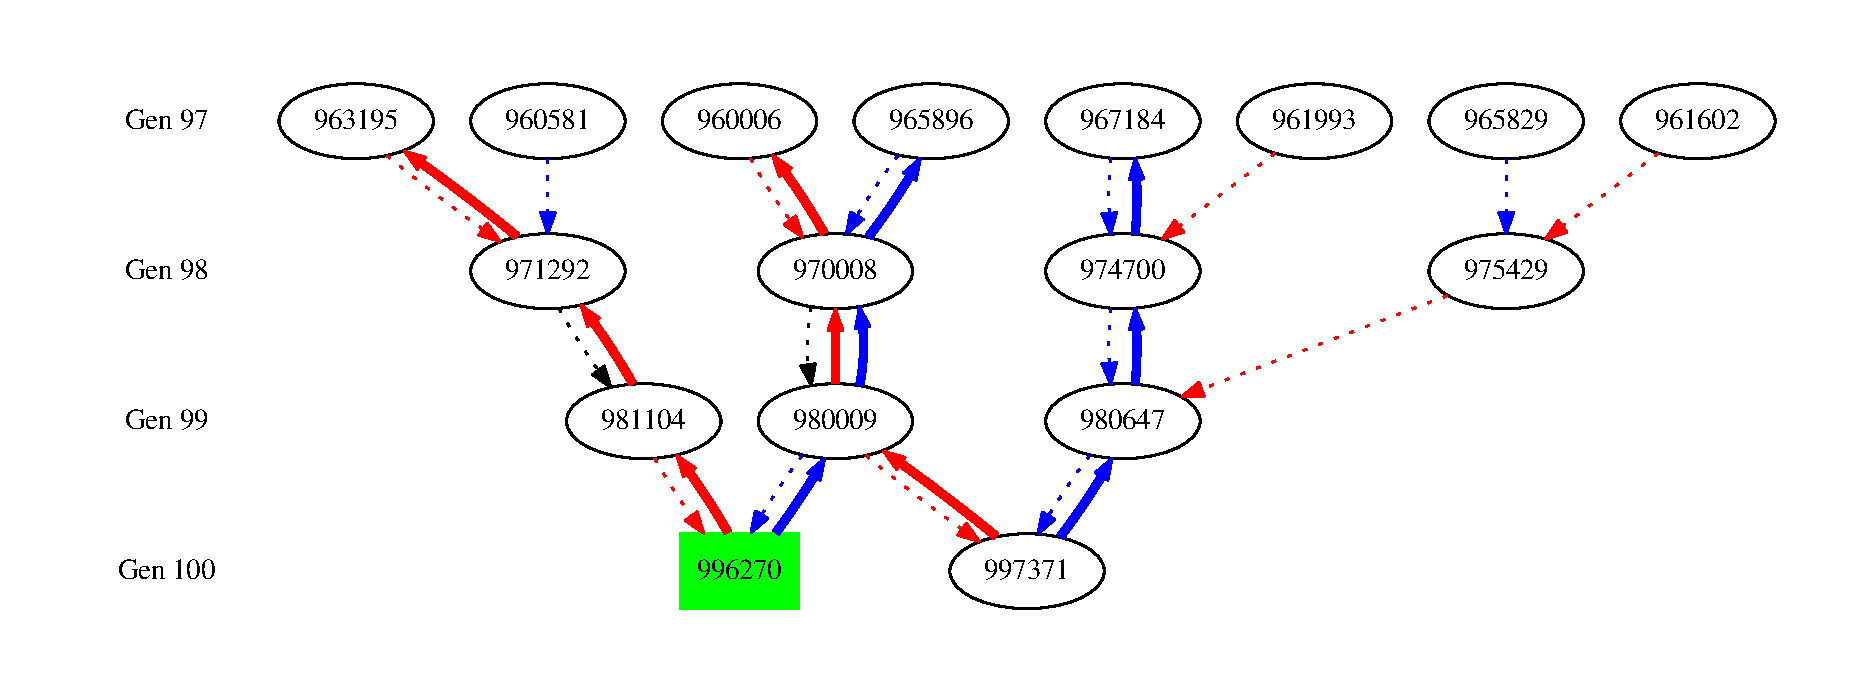
\includegraphics[width=\textwidth]{XO_path_example}
 \caption{Part of the root and non-root ancestry paths of two individuals in the final generation of a run. Dotted arrows represent transformations: blue for root crossover, red for non-root crossover, black for reproduction. Solid arrows represent the root and non-root ancestry paths, with blue for the root ancestry path and red for non-root ancestry path. Solid blue paths traverse dotted blue and black edges, and solid red paths traverse dotted red and black edges. The individual marked by the green box is the most fit individual in the final generation of this run. Note that the reproduction edge from 970008 to 980009 is part of both the root ancestry path for node 996270 and the non-root ancestry path for node 997371.}
 \label{fig:XO_path_example}
\end{figure}

Before describing several questions and queries that we performed using graph databases, we need to define the concept of \emph{the root ancestry line}. The root line of a specified individual $n$ is the path from $n$ to some individual in the initial population, following only root parent crossover transformations and all single parent transformations (elitism, reproduction, and mutation). The non-root line follows the non-root crossover transformation as well as the single parent transformations. Figure~\ref{fig:XO_path_example} illustrates these ideas.

The following, then, are some of the questions we asked of the database:
\begin{itemize}
\item \emph{How many individuals in the initial generation have any root parent descendants in the final generation?} (Section~\ref{sec:numberInitialIndividualsWithDescendants})
\item \emph{How often do mutations improve fitness? Also, how often do crossovers improve fitness, where the root parent is more fit than the non-root parent, and vice versa?} (Section~\ref{sec:effectivenessMutationCrossover})
\item \emph{What does the fitness of the ``winning'' root parent ancestry line look like over time?} (Section~\ref{sec:WinningRootLineFitness})
\item \emph{Do a group of individuals have a common root parent ancestor and what is the latest generation where such an ancestor occurs?} (Section~\ref{sec:MostRecentCommonAncestor})
\end{itemize}

\subsection{Number of Initial Individuals With Final Generation Descendants}
\label{sec:numberInitialIndividualsWithDescendants}

To answer the first question, how many individuals from the initial generation have descendants in the final generation, we used the query in Query~\ref{query:InitialIndividualsWithDescendants}. The \texttt{MATCH} statement describes that \texttt{startNode} and \texttt{endNode} are individuals in generation one and one hundred respectively. The path between them must consist of only elitism, reproduction, mutation, or root parent crossover transformations and must have length 99. The \texttt{RETURN} statement returns the ID and penalized fitness of every individual in the initial generation that fit the criteria. An example response from this query is presented in Table \ref{tab:descendantsTable}.

\begin{Query}
\begin{verbatim}
MATCH (startNode:Individual {generation: 1})
   -[:ELITISM|PARENTOF|MUTANTOF|ROOT_XOOF*99]->
   (endNode:Individual {generation:100})
RETURN DISTINCT id(startNode), startNode.penalizedFitness;
\end{verbatim}
\caption{Cypher query to generate the set of individuals in the initial generation that have root descendants in the final generation.}
\label{query:InitialIndividualsWithDescendants}
\end{Query}

\begin{table}[tb]
\begin{center}
\begin{tabular}{|r|r|}
    \hline
    \textbf{Individual ID} & \textbf{Penalized Fitness} \\ \hline
    2595 & 38.98 \\
    3325 & 40.36 \\
    \hline
\end{tabular}
\caption{List of individuals in the initial generation of the 10K run which produced root descendants in the final generation.}
\label{tab:descendantsTable}
\end{center}
\end{table}

This data demonstrates that, at least in this specific instance, all 10,000 individuals in the final generation can be traced back along their root parent line to only two individuals in the initial generation. This, in support of data gathered by McPhee and Hopper \cite{mcphee1999analysis}, indicates that the percentage of initial individuals with direct descendants in the final generation is extremely small. Furthermore, while neither of these individuals had the best initial fitness (24.18), both do appear in the top 5\% of first generation individuals. Whether this high fitness rate is consistent across multiple runs is unclear and is worth further exploration.

\subsection{Effectiveness of Mutation and Crossover}
\label{sec:effectivenessMutationCrossover}

To determine the effectiveness of mutation and crossover in producing more fit offspring, we wrote the queries in Query~\ref{query:effectivenessMutationCrossover}. These two queries specifically identified the total number of crossovers and the number of root crossovers where the child was more fit than either parent and the root parent was more fit than the non-root parent. Note that the \texttt{MATCH} clause allows relationships in both directions, so the pattern \texttt{(r)-->(c)<--(n)} matches cases where there is a relationship from node \texttt{r} to node \texttt{c}, and a relationship from node \texttt{n} to node \texttt{c} as well. In the query, we further qualify these two edges, requiring one to be a root parent relationship, and the other a non-root parent relationship. The \texttt{WHERE} clause allows us to filter out undesired matches, in this case limiting us to instances where the child's fitness is better than the root parent's, and the root parent's is better than the non-root parent's.

\begin{Query}
\begin{verbatim}
// Count total number of crossovers.

MATCH (rootParent)-[:ROOT_XOOF]->(child)
   <-[:NONROOT_XOOF]-(nonRootParent)
RETURN COUNT(DISTINCT child);

// Count total number of crossovers where the child is more
// fit than the root parent, which is more fit than the
// non-root parent.

MATCH (rootParent)-[:ROOT_XOOF]->(child)
   <-[:NONROOT_XOOF]-(nonRootParent)
WHERE child.penalizedFitness < rootParent.penalizedFitness 
   AND rootParent.penalizedFitness 
                          < nonRootParent.penalizedFitness
RETURN COUNT(DISTINCT child);
\end{verbatim}
\caption{Cypher queries to compute the total number of crossover events, and the number where the child's fitness is better than the root parent's fitness, which is in turn better than the non-root parent's fitness.}
\label{query:effectivenessMutationCrossover}
\end{Query}

Given the counts from these two queries, we can compute the proportion of crossovers where the child was more fit than the root parent, which was more fit than the non-root parent. The queries for the other two cases, where mutation led to a more fit offspring, and where non-root crossover led to a child which was more fit than either parent and non-root parent was more fit than the root parent, had similar structures. The results of these query may be seen in Figure \ref{fig:improvedFitness}.

\begin{figure}[p]
 \centering
 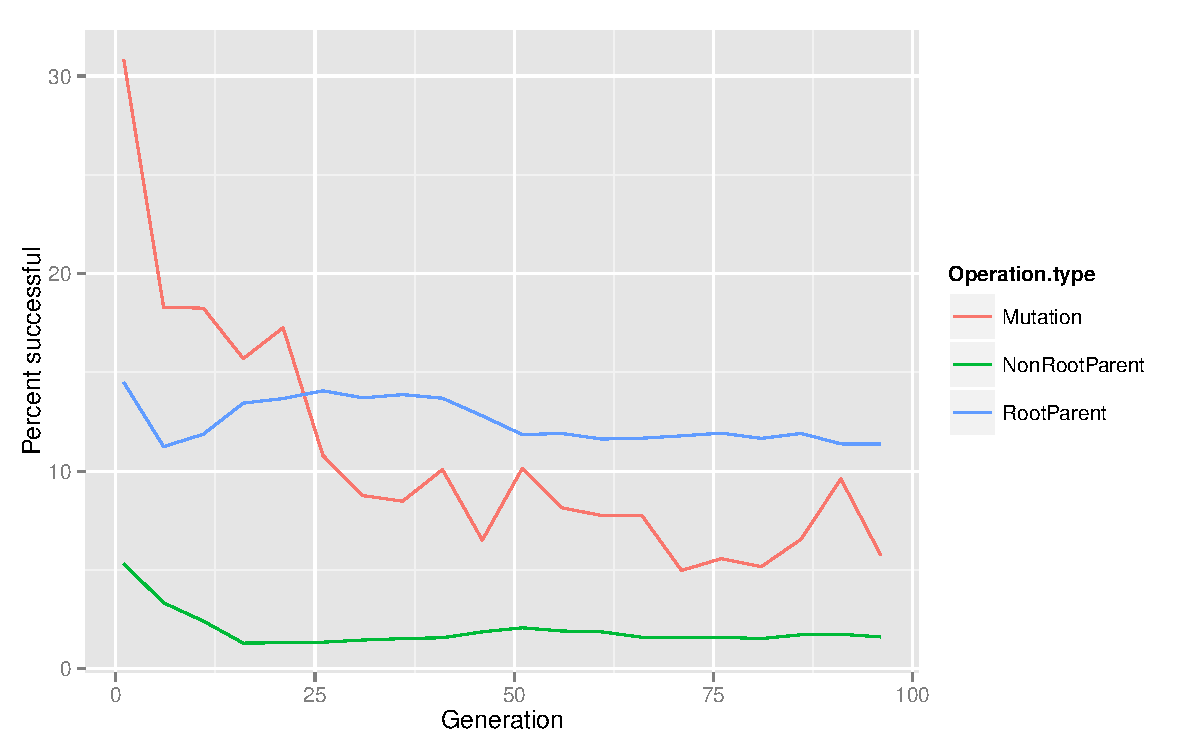
\includegraphics[height=0.63\textwidth]{Blocked_success_percentages}
 \caption{Percentage of cases where the child is fitter than the parent in 10K run.}
 \label{fig:improvedFitness}
\end{figure}

The data in Figure~\ref{fig:improvedFitness} is from a single run with 10,000 individuals; we also applied these same queries on three 1,000 individual runs to obtain the very similar graph in Figure~\ref{fig:improvedFitness1K}. In the first generations, mutation produced children that were better than their parents over 30\% of the time. As time progressed, the success of mutation decreased dramatically, dropping as low as 2\%. On the other hand, the crossover percentages stayed relatively constant with the exception of the first ten generations of non-root crossover. Notice that the crossover variances were very small, meaning that the performance of crossover is stable over time. 

\begin{figure}[p]
 \centering
 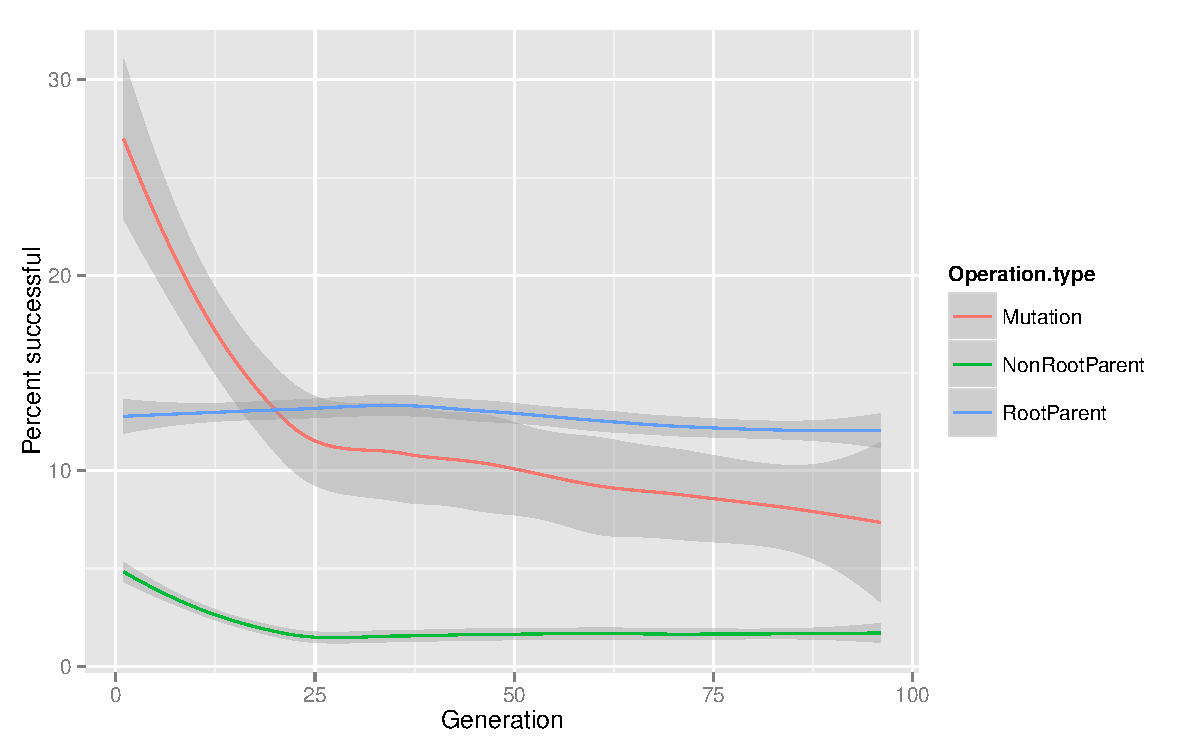
\includegraphics[height=0.63\textwidth]{Percent_successful_Axiom_1K_runs}
 \caption{Percentage of cases where the child is fitter than the parent in three 1K runs. Shadows indicate the variance across the three runs.}
 \label{fig:improvedFitness1K}
\end{figure}

\subsection{Winning Root Ancestry Line Fitness}
\label{sec:WinningRootLineFitness}

We used the query in Query~\ref{query:WinningRootLineFitness} to find the fitnesses along the root ancestry line from the best individual in the final population. A similar query generated fitness information along the non-root parent line; these are graphed in Figure~\ref{fig:rootVsNonrootFitness}. As can be seen, while root parent fitness steadily decreases over time, no such pattern exists for non-root fitness. This implies that the root lineage is far more important in determining the overall success of a specific individual than the non-root lineage.

\begin{Query}
\begin{verbatim}
START winner=node(996270)
MATCH (winner)
       <-[:ELITISM|PARENTOF|MUTANTOF|ROOT_XOOF*0..]-(parent)
RETURN parent.generation, parent.penalizedFitness, 
                                     parent.fitness, "Root";
\end{verbatim}
\caption{Cypher query to compute the fitnesses along the root ancestry line from the best individual in the final population.}
\label{query:WinningRootLineFitness}
\end{Query}

\begin{figure}[tb]
 \centering
 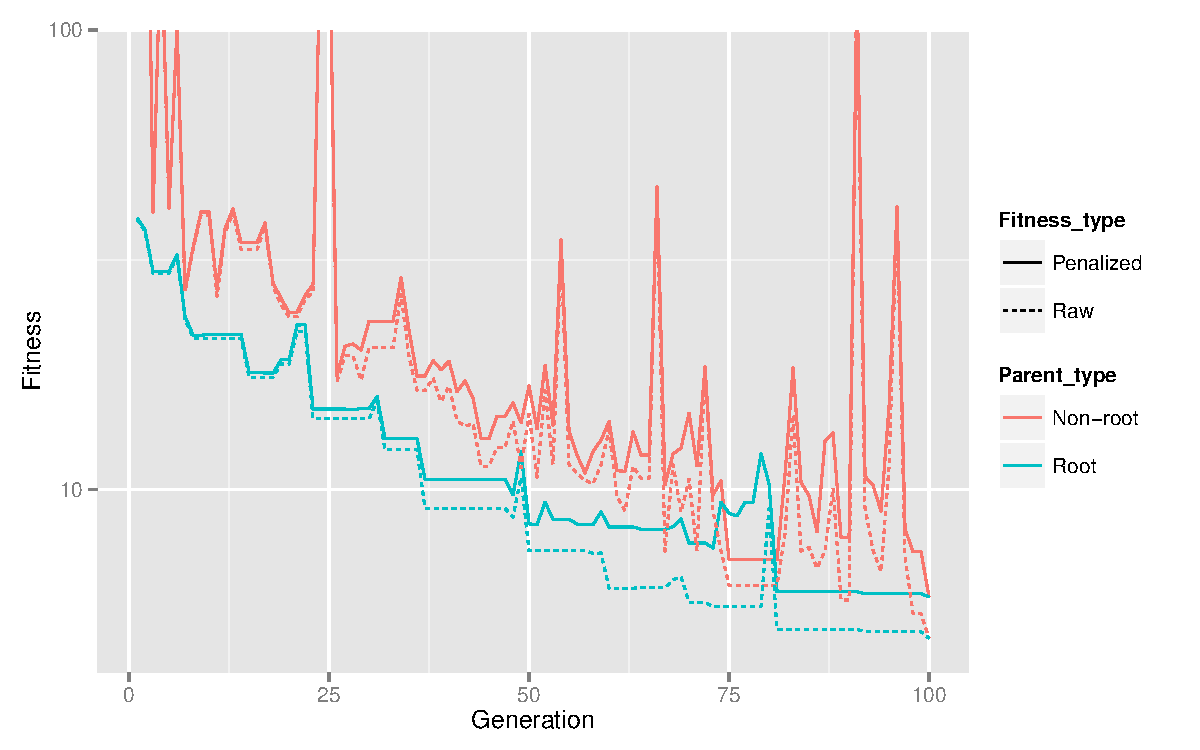
\includegraphics[height=0.68\textwidth]{Combined_fitness_over_time}
 \caption{Root versus non-root fitness in ancestry of best tree from final generation of a 10K run. The raw fitness is the fitness before the size penalty is added. A logarithmic scale has been applied to the fitness axis.}
 \label{fig:rootVsNonrootFitness}
\end{figure}

\subsection{Most Recent Common Ancestor}
\label{sec:MostRecentCommonAncestor}

For our fourth and final question, finding a common ancestor of entire last generation, we executed the query in Query~\ref{query:MostRecentCommonAncestor}. An example of a common ancestry graph can be seen in Figure \ref{fig:ancestryGraph}. In finding a common ancestor, we can assume that this ancestor carries certain positive traits. This information may be relevant in determining if traits other than fitness give an individual an increased chance of survival. In the 10,000 individual run, two distinct clades were produced. One clade flourished, accounting for 99.76\% of the final population (including the individuals in Figure~\ref{fig:ancestryGraph}), while the second clade consisted of only 24 individuals in the final generation. These two clades are descended from the individuals presented in Table~\ref{tab:descendantsTable}. Descendants of the more fit individual profoundly predominated, and given more time, the second clade most likely would have gone extinct. 

\begin{Query}[t]
\begin{verbatim}
MATCH (child:Individual {generation: 100})
   <-[:ELITISM|PARENTOF|MUTANTOF|ROOT_XOOF*0..]-(parent)
   <-[rel:ELITISM|PARENTOF|MUTANTOF|ROOT_XOOF]-(grandparent)
RETURN DISTINCT id(parent), type(rel), id(grandparent);
\end{verbatim}
\caption{Cypher query to find the set of common root ancestors of all the individuals in the final generation.}
\label{query:MostRecentCommonAncestor}
\end{Query}

\begin{figure}[tb]
 \centering
 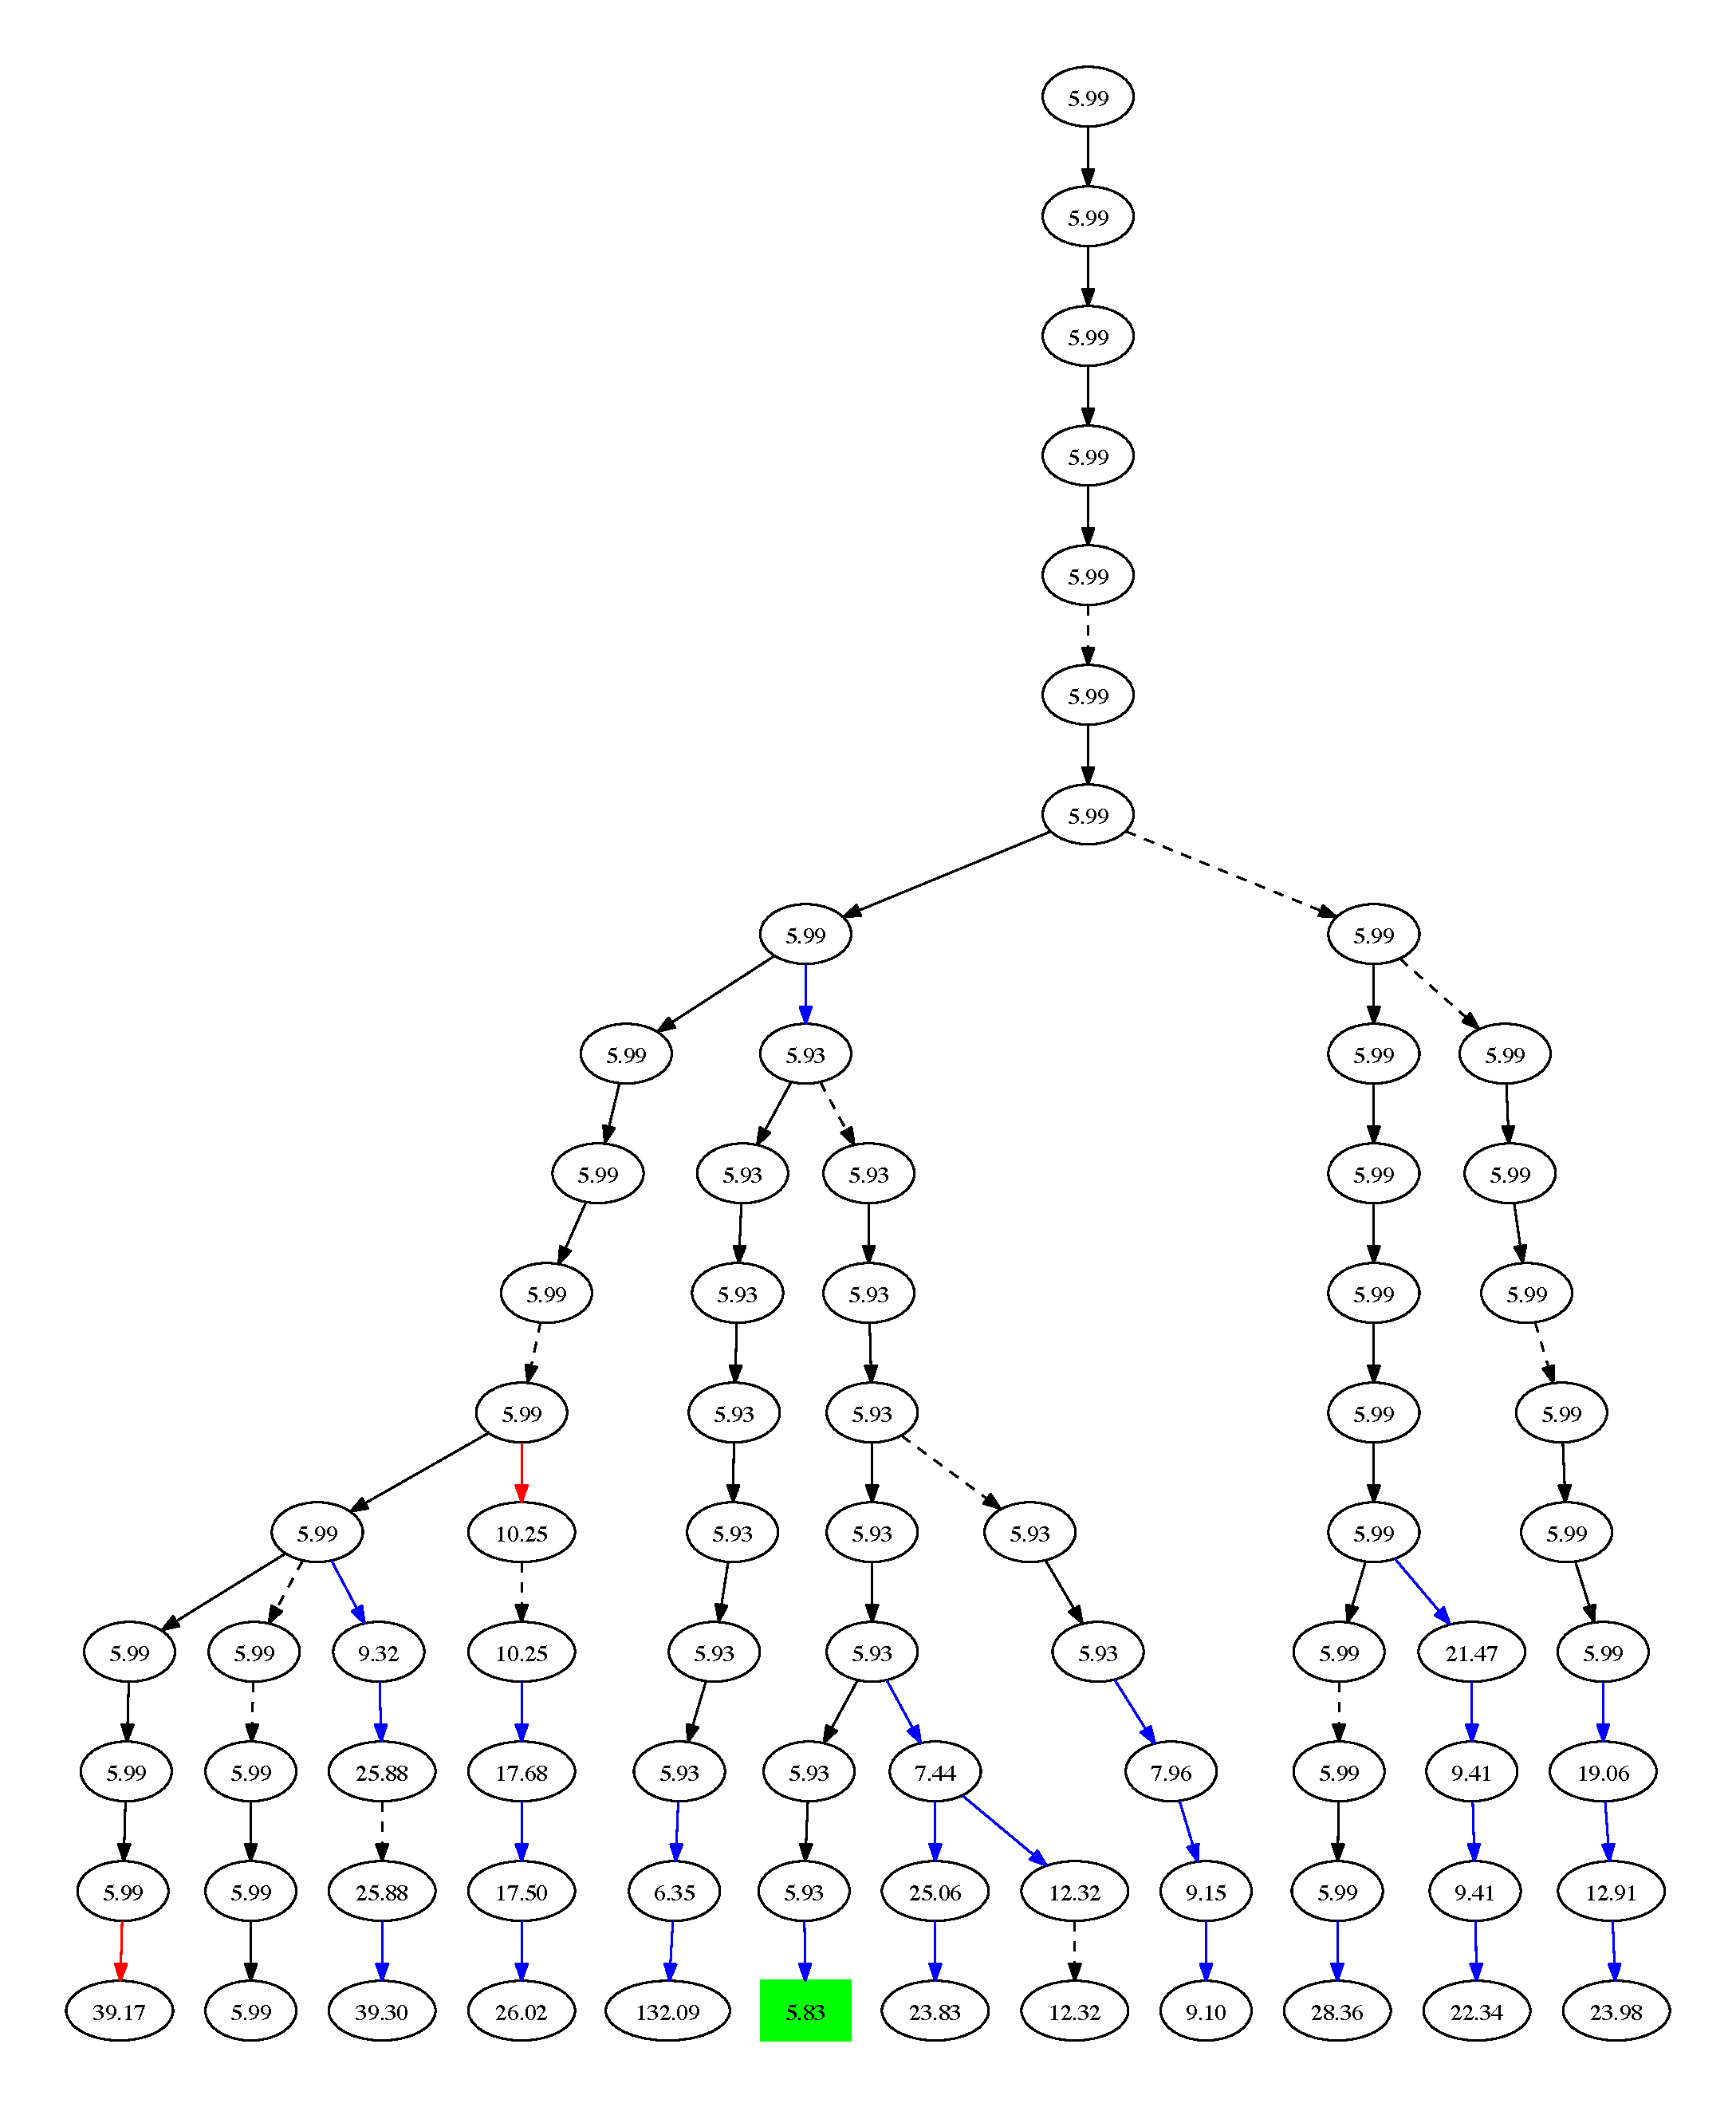
\includegraphics[width= \textwidth]{subset_confluence_trimmed}
 \caption{Results of finding the common ancestor  between the ``winner'',  highlighted by a green box, and 11 of its close relatives. Mutation relationships are highlighted by red arrows. Crossovers are blue arrows. Reproduction is a dotted black line and elitism is a solid black line. Note that this is an abbreviated ancestry stopping at generation 84; the common line continues back all the way to generation 1.}
 \label{fig:ancestryGraph}
\end{figure}

\section{Conclusions} \label{sec:conclusion}

A critical point is that graph databases like Neo4j don't make anything possible that was once impossible; they instead make these things vastly simpler and allow open-ended exploration. Each of the queries and questions we've discussed could be handled by, for example, special purpose code added to the evolutionary system to capture that specific information. Many, if not most, of these questions have no doubt been addressed in a piecemeal fashion by previous research. Researchers observed~\cite{mcphee1999analysis} nearly 15 years ago that root parent lineages were significant, and that these lineages quickly coalesced into a shared common ancestor, but that was using a custom system to track that data, and there has been limited follow-up by others since then. We suspect a significant reason for the lack of similar work is simply the effort required to collect and analyze the substantial amount of data this entails, and the lack of good tools to simplify that process.

Now that we have access to a plethora of data from GP runs, we are capable of potentially deducing new, important patterns. For future research, we have identified several topics to possibly pursue.

One topic which may benefit from further investigation is the percentage of effective transformations where the child is more fit than its parent or parents. We could, for example, dynamically tune mutation and crossover percentages over time to increase the likelihood of generating effective transformations. Additionally, we could also investigate the effect of forcing the root parent to have a better fitness than the non-root parent, since the data in Figures~\ref{fig:improvedFitness}~and~\ref{fig:improvedFitness1K} clearly indicates that offspring from such a combination have a much higher probability of having improved fitness.

Another potential route to explore how often long-term persistent clades exist. It would also be interesting to see if and when clades interbreed, or if they are completely separate species. If there is any interbreeding, this would allow exploration into how interbreeding contributes to the overall fitness of the clade.

A final area for further investigation is to analyze the fitness over time of the ``winning'' lineage. In Figure~\ref{fig:rootVsNonrootFitness}, we saw several areas were the fitness became worse before becoming better. Although spikes of poor fitness do not happen prior to all improvements, these spikes do happen frequently enough to be potentially significant. Investigation into the characteristics of changes in individuals in these spikes could lead to a better understanding of how improvements in fitness occur.

There are many other questions that could be potentially addressed because of the sheer amount of data Neo4j allows us to collect and process. So far we have done very few runs, and only on a single test problem. Doing more runs, and exploring a variety of problems would help us understand how representative some of these results are.

In summary, while this work has demonstrated that Neo4j is a useful tool in recording and analyzing data collected from genetic programming systems, there is much further work to be done with this information.

\section*{Acknowledgements}

David's work was supported by the Morris Academic Partners program at the University of Minnesota, Morris. Many thanks to Nicholas Cornhill and Emma Ireland for their early help in connecting evolutionary computation systems to Neo4j.

\pagebreak

\bibliographystyle{acm}
\bibliography{MICS_2014}

\end{document}
